\chapter{VOTable format definition} % (fold)
\label{cha:votable_format_definition}

The VOTable is the main data interchange standard existing in the VO,
and is an IVOA Recommendation since 2004. Its formal definition can be
found in~\cite{2004votfdivoav0811O}, or in the IVOA Documents
site\urlnote{http://www.ivoa.net/Documents/latest/VOT.html}. However, we
will provide in this appendix a brief description of the VOTable format
which also aims to illustrate some parts of that document.

\invisiblenote
{The reason for the use of a common interchange format in astrophysics
was already addressed when the FITS format ---see
appendix~\ref{cha:description_of_the_fits_file_format}--- was
defined: only with common data interchange formats can different tools,
on different workstations, be used on data coming from different
sources.

Once FITS limitations were evident, and the industry commenced to
converge on XML as a common data format with interesting properties both
for hierarchical and tabular data, and the Astrophysical Virtual
Observatory prototype was in development, the CDS proposed an XML
document definition~\cite{2000ASPC..216...83O}. This initial proposal
was the seed which later evolved to take the form of the VOTable.

\todo{Move the two paragraphs above to the main \texttt{introvo}
article.}}

\section{VOTable DTD} % (fold)
\label{sec:votable_dtd}

The initial definition of the VOTable, version 1.0, was made in terms of
an XML Document Type Definition (DTD), which can be found in listing
\ref{lst:VOTableDTD}. This document specifies \texttt{ELEMENT}s, which
are the tags that can be used to markup data, and which tags can be
included, and how many times, within any other tag; and
\texttt{ATTLIST}s, or attribute lists, which are the attributes that can
further refine a tag being applied to a piece of data.

\lstinputlisting[
	language=XML,
	caption={[VOTable DTD] VOTable 1.0 Document Type Definition.},
	label=lst:VOTableDTD,
	firstline=1,
	lastline=64,
	float
]
{dtd/votable.dtd}
\lstinputlisting[
	language=XML,
	caption={VOTable 1.0 DTD: continued},
	firstline=65,
	lastline=128,
	nolol,
	float
]
{dtd/votable.dtd}
\lstinputlisting[
	language=XML,
	caption={VOTable 1.0 DTD: continued},
	firstline=130,
	nolol,
	float
]
{dtd/votable.dtd}

% section votable_dtd (end)

\section{VOTable XML Schema Definition} % (fold)
\label{sec:votable_xml_schema_definition_xsd_}

A new version of the VOTable, version 1.1, was a little bit more
restrictive on what is an acceptable VOTable, by means of an XML Schema
Definition (XSD). The XML schema can be seen in
listing~\ref{lst:VOTableXSD}.

\lstinputlisting[
	language=XML,
	caption={[VOTable XML Schema] VOTable XML Schema.
	         Notice the version numbering from the first
	         schema definition, compatible with the DTD
	         version, to the latest XML Schema.},
	label=lst:VOTableXSD,
	firstline=1,
	lastline=74,
	float
]
{xsd/VOTable-1.1.xsd.xml}
\lstinputlisting[
	language=XML,
	caption={VOTable XML Schema: cont.},
	nolol,
	firstline=76,
	lastline=144,
	float
]
{xsd/VOTable-1.1.xsd.xml}
\lstinputlisting[
	language=XML,
	caption={VOTable XML Schema: cont.},
	nolol,
	firstline=146,
	lastline=215,
	float
]
{xsd/VOTable-1.1.xsd.xml}
\lstinputlisting[
	language=XML,
	caption={VOTable XML Schema: cont.},
	nolol,
	firstline=216,
	lastline=286,
	float
]
{xsd/VOTable-1.1.xsd.xml}
\lstinputlisting[
	language=XML,
	caption={VOTable XML Schema: cont.},
	nolol,
	firstline=288,
	lastline=366,
	float
]
{xsd/VOTable-1.1.xsd.xml}
\lstinputlisting[
	language=XML,
	caption={VOTable XML Schema: cont.},
	nolol,
	firstline=368,
	lastline=443,
	float
]
{xsd/VOTable-1.1.xsd.xml}
\lstinputlisting[
	language=XML,
	caption={VOTable XML Schema: cont.},
	nolol,
	firstline=445,
	float
]
{xsd/VOTable-1.1.xsd.xml}

The additional restrictions over the VOTable 1.0 standard (those defined by the DTD) are, among others:

\begin{itemize}
	\item \texttt{ucdType} validates against UCD1 or UCD1+
	Unified Content descriptors, allowing the rejection of
	VOTables with UCDs using not allowed characters.
	
	\item \texttt{astroYear} validates against Besselian or
	Julian years' specifications (e.g., \texttt{J2000},
	\texttt{B1950}, but not \texttt{2000} or \texttt{F2000}).
	
	\item \texttt{arrayType} validates against the
	specification of fixed or variable array sizes (e.g.,
	\texttt{12x23x*}, but not \texttt{12 by 23}).
	
	\item \texttt{precType} validates against the syntax for
	precision specification (e.g., \texttt{F10}, \texttt{E5} or
	\texttt{5}, but not \texttt{12F}).
\end{itemize}

And the use of XML Schema native data types allows an easier
specification of data bounds, such as \texttt{xs:nonNegativeInteger},
or of date and time time stamps with \texttt{xs:dateTime}.


% section votable_xml_schema_definition_xsd_ (end)

\section{VOTable structure} % (fold)
\label{sec:votable_structure}

Independently of whether a VOTable XML document specifies its document
type via a DTD or the VOTable XML Schena, its structure can be seen in
figure~\ref{fig:fig_VOTable11}.

\begin{figure}[tbp]
	\centering
		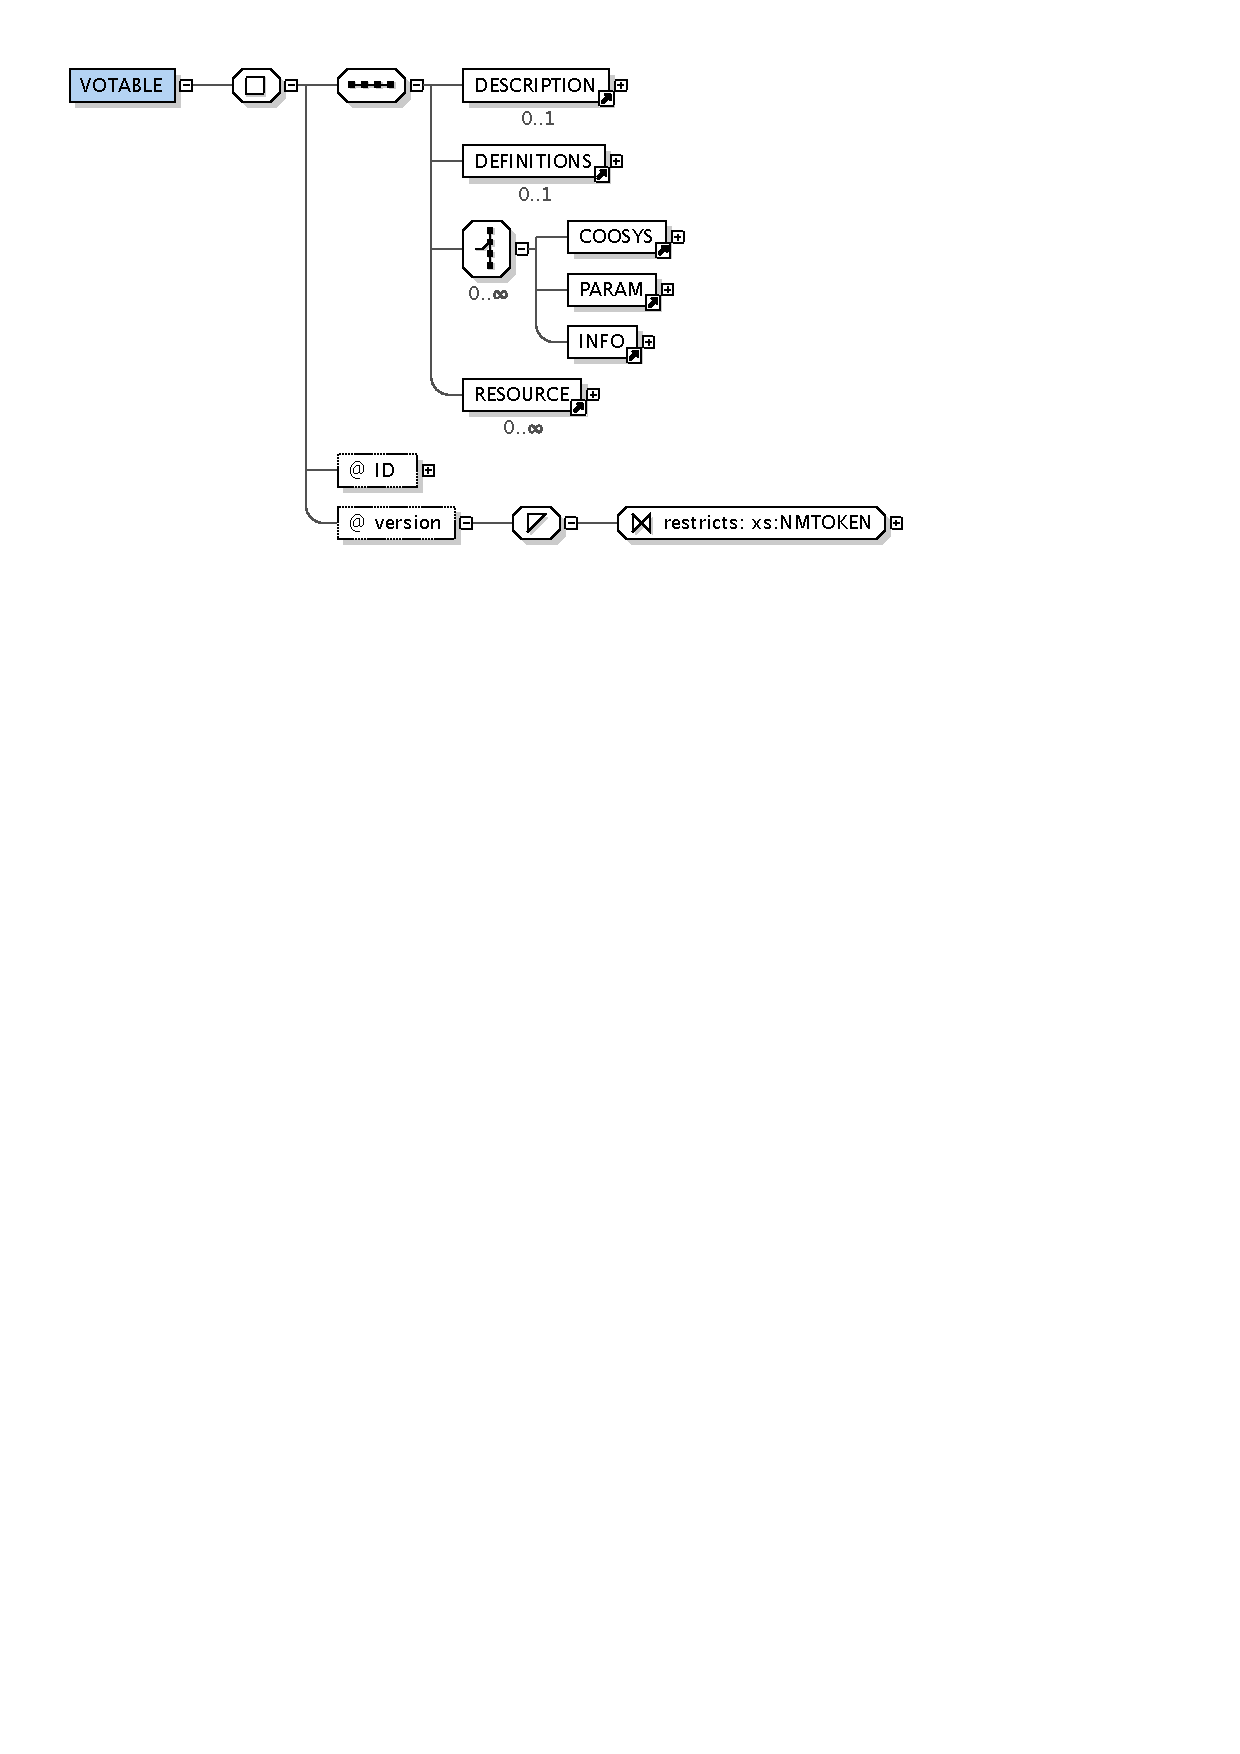
\includegraphics[width=\columnwidth]{fig/VOTable11.pdf}
	\caption[Elements of the \xmltag{VOTABLE}]
	{
		VOTable high level structure, seen as elements of the
        \xmltag{VOTABLE}. Inside the root \xmltag{VOTABLE}, a
        \xmltag{DESCRIPTION} can be used to describe in human readable
        form the contents of a particular VOTable. After that, in
        VOTable 1.0 the \xmltag{DEFINITIONS} could be used to provide
        global information, coordinate systems, and params. In VOTable
        1.1 it is recommended to specify global coordinate system
        definitions via the \xmltag{COOSYS} right below the
        \xmltag{VOTABLE}, followed by the \xmltag{PARAM} (for specifying
        fixed values, such as a value for the Hubble constant, a global
        instrumental parameter, or similar constant values affecting the
        whole VOTable) and the \xmltag{INFO} for documentation. Those
        tags can be used as many times as needed, and after them any
        number of \xmltags{RESOURCE} can appear as many times as needed,
        specifying actual data resources. If more than one
        \xmltags{COOSYS} are specified, their \texttt{ref} attribute
        must be set so that the relevant coordinate system can be
        referenced from within a \xmltag{TABLE}.
		\oxygenxml
	}
	\label{fig:fig_VOTable11}
\end{figure}


A VOTable, then, is an XML document whose root element is the
\xmltag{VOTABLE}, and which might hold inside a \xmltag{DESCRIPTION}, a
\xmltag{DEFINITIONS}\footnote{This tag is deprecated in the version 1.1
of the VOTable definition, which has made the \xmlopen{COOSYS},
\xmlopen{PARAM} and \xmltags{INFO} first-class citizens under the
\xmltag{VOTABLE}.}, and a \xmltag{COOSYS}. More importantly, a VOTable
can contain several \xmltags{RESOURCE}, each of one could contain any
number of \xmlopen{TABLE} and/or \xmltags{RESOURCE}.
Figure~\ref{fig:fig_VOTableResourceTag} shows the structure of a
\xmltag{RESOURCE}, while figure~\ref{fig:fig_VOTableTableTag} shows the
structure of a \xmltag{TABLE}.

\subsection{The \xmltag{COOSYS}} % (fold)
\label{sub:the_coosys_tag}

The celestical coordinate systems to be used throughout a particular
VOTable are specified by the \xmltag{COOSYS}. Its structure is
illustrated by figure~\ref{fig:fig_VOTableCoosysTag}.

The valid values for the \texttt{system}
attribute of the \xmltag{COOSYS} are shown in
table~\ref{tab:coordinateTypes}, with small descriptions of the different coordinate systems which can be specified.

\begin{table}
	\caption[Valid \texttt{encodingType} attributes]{
		Meaning of the different valid values for attributes of the
		\texttt{encodingType} data type.
	}
	\begin{smallertabular}{rp{9.75cm}}
	
	\textbf{\emph{system} type} & \textbf{Description}\\\midrule
	
	\texttt{ICRS} & Coordinates are given in the International
	Celestial Reference System.\\\addlinespace
	
	\texttt{eq\_FK5} & Equatorial coordinates, using 
	the Fifth General Catalogue as reference frame.\\\addlinespace
	
	\texttt{eq\_FK4} & Equatorial coordinates, using 
	the Fourth General Catalogue as reference frame.\\\addlinespace
	
	\texttt{ecl\_FK5} & Ecliptic coordinates, using 
	the Fifth General Catalogue as reference frame.\\\addlinespace
	
	\texttt{ecl\_FK4} & Ecliptic coordinates, using 
	the Fourth General Catalogue as reference frame.\\\addlinespace
	
	\texttt{galactic} & Galactic coordinates, using the
	galactic reference frame, with the Sun at the
	centre, and the line in the galactic plane between the Sun
	and the centre of the Milky way used as baseline for
	determining galactic latitude and longitude.\\\addlinespace
	
	\texttt{supergalactic} & Supergalactic coordinates,
	similar to galactic coordinates, but where the
	preferential plane is that containing the barycentres of the 
	the Virgo, Perseo-Pisces, and Great Attractor galaxy 
	clusters, while the preferential line is the intersection
	of the plane of the Milky Way with the supergalactic
	plane.\\\addlinespace
	
	\texttt{barycentric} & Coordinates co-moving with the
	Sun, but with time measurements free from relativistic 
	corrections due to the presence of gravity. \\\addlinespace
	
	\texttt{geo\_app} & Coordinates refer to the Earth
	longitude and latitude.
	\\\addlinespace
	
	\texttt{xy} & Corresponds to a user-defined coordinate
	system, similar to the \texttt{alpha} and \texttt{beta}
	coordinates in the IRAM New Control System.
	\end{smallertabular}
	\label{tab:coordinateTypes}
\end{table}

In the case of the \texttt{eq\_FK?} and \texttt{ecl\_FK?} coordinate
systems, the \texttt{equinox} attribute is used to fix the systems
(with default vaule \texttt{J2000} for \texttt{*\_FK5}, and
\texttt{B1950} for \texttt{*\_FK4}). If necessary, the \texttt{epoch}
attribute can provide the epoch for the positions.

\begin{figure}[tbp]
	\centering
		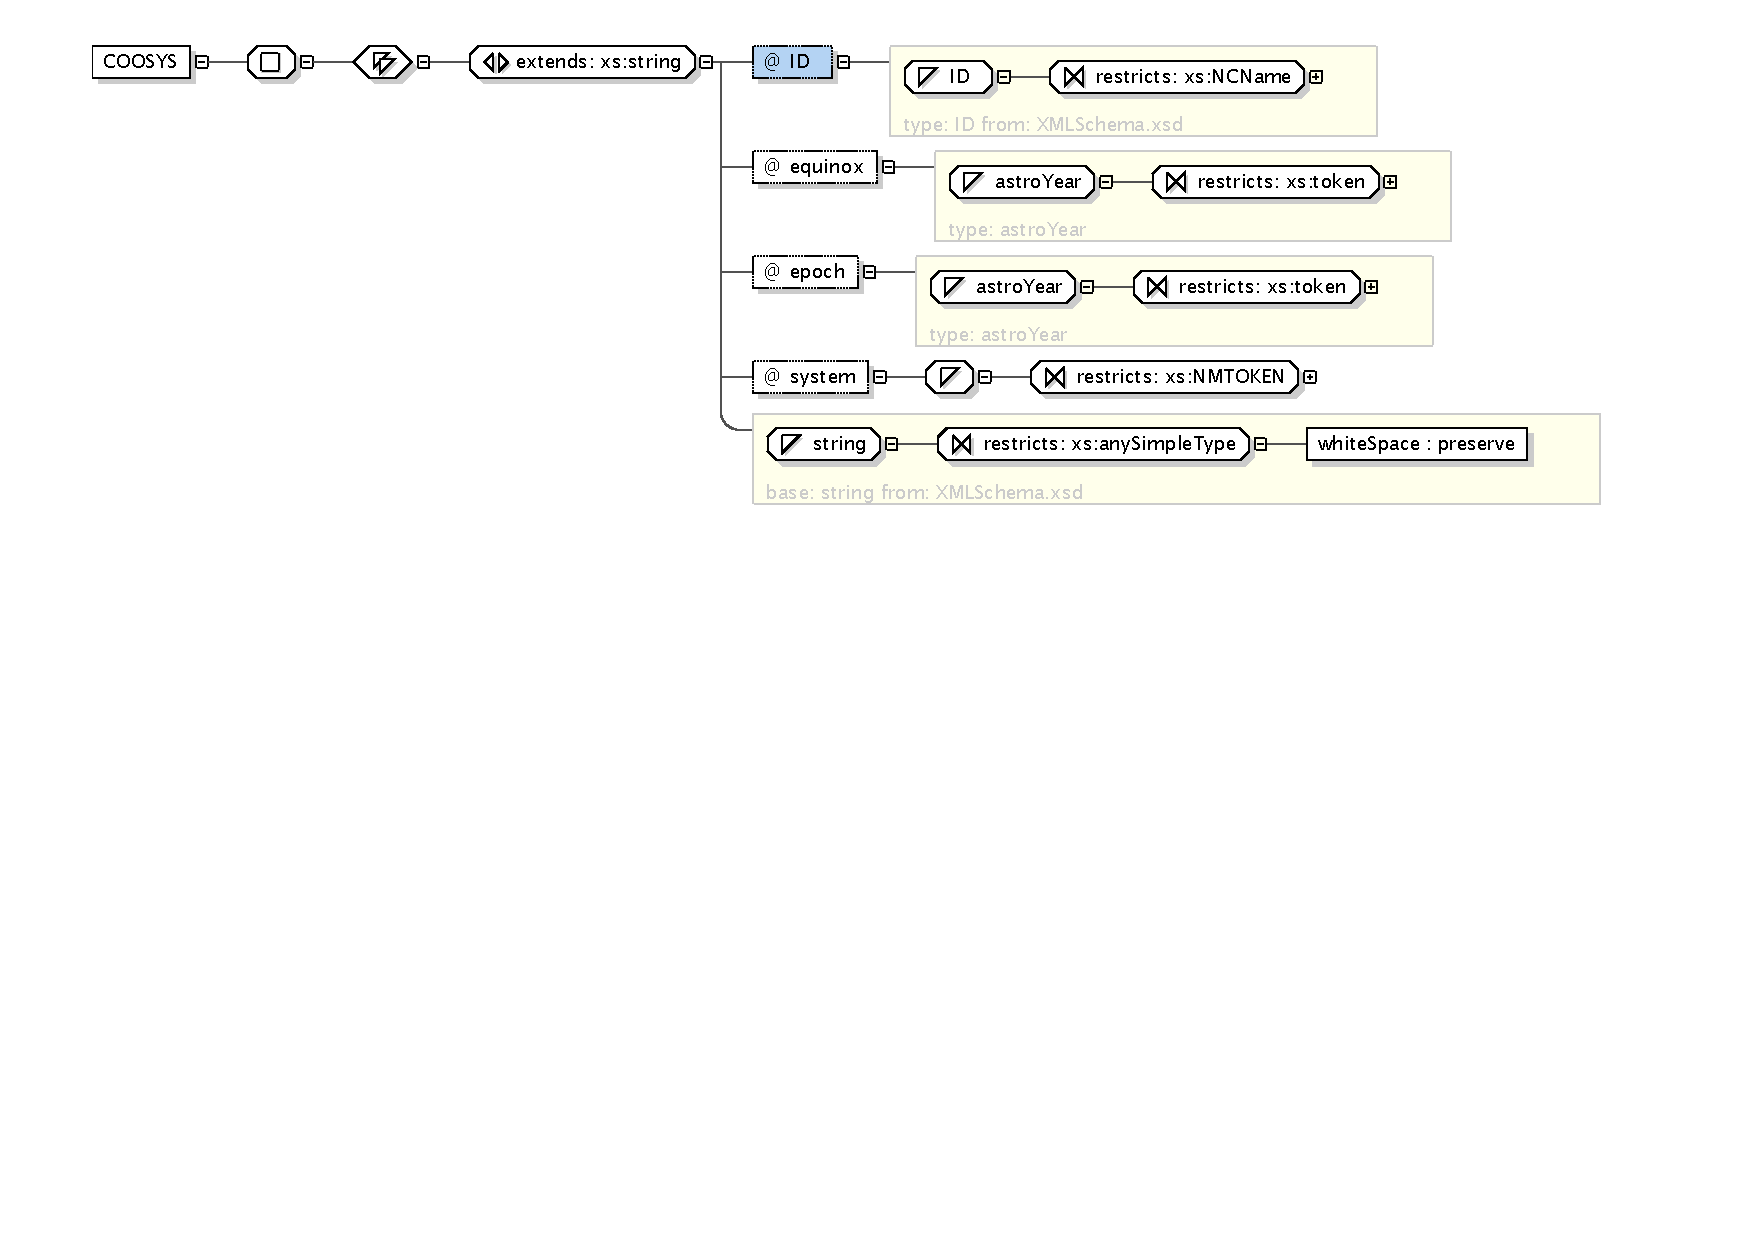
\includegraphics[width=\columnwidth]{fig/VOTableCoosysTag.pdf}
	\caption[Attributes of the \xmltag{COOSYS}]{
		The \xmltag{COOSYS} attributes, with data types.
		The \texttt{ID} attribute can be used in \texttt{ref} attributes
		in coordinate fields in order to establish a particular
		coordinate system, if more than one \xmltags{COOSYS} are
		specified. Both the \texttt{epoch} and \texttt{equinox}
		attributes correspond to an \texttt{astroYear} data type.
	}
	\label{fig:fig_VOTableCoosysTag}
\end{figure}

In the future, the \xmltag{COOSYS} might be deprecated in favour of an
STC\cite{2007stc..ivoa.....R} serialisation (complete or simplified).

% subsection the_coosys_tag (end)

\subsection{The \xmltag{RESOURCE}} % (fold)
\label{sub:the_resource_tag}

\xmltags{RESOURCE} provide data values, preceded with a description, of
some logically independent data structure. We can see the structure of
a \xmltag{RESOURCE} in figure~\ref{fig:fig_VOTableResourceTag}.

\begin{figure}[tbp]
	\centering
		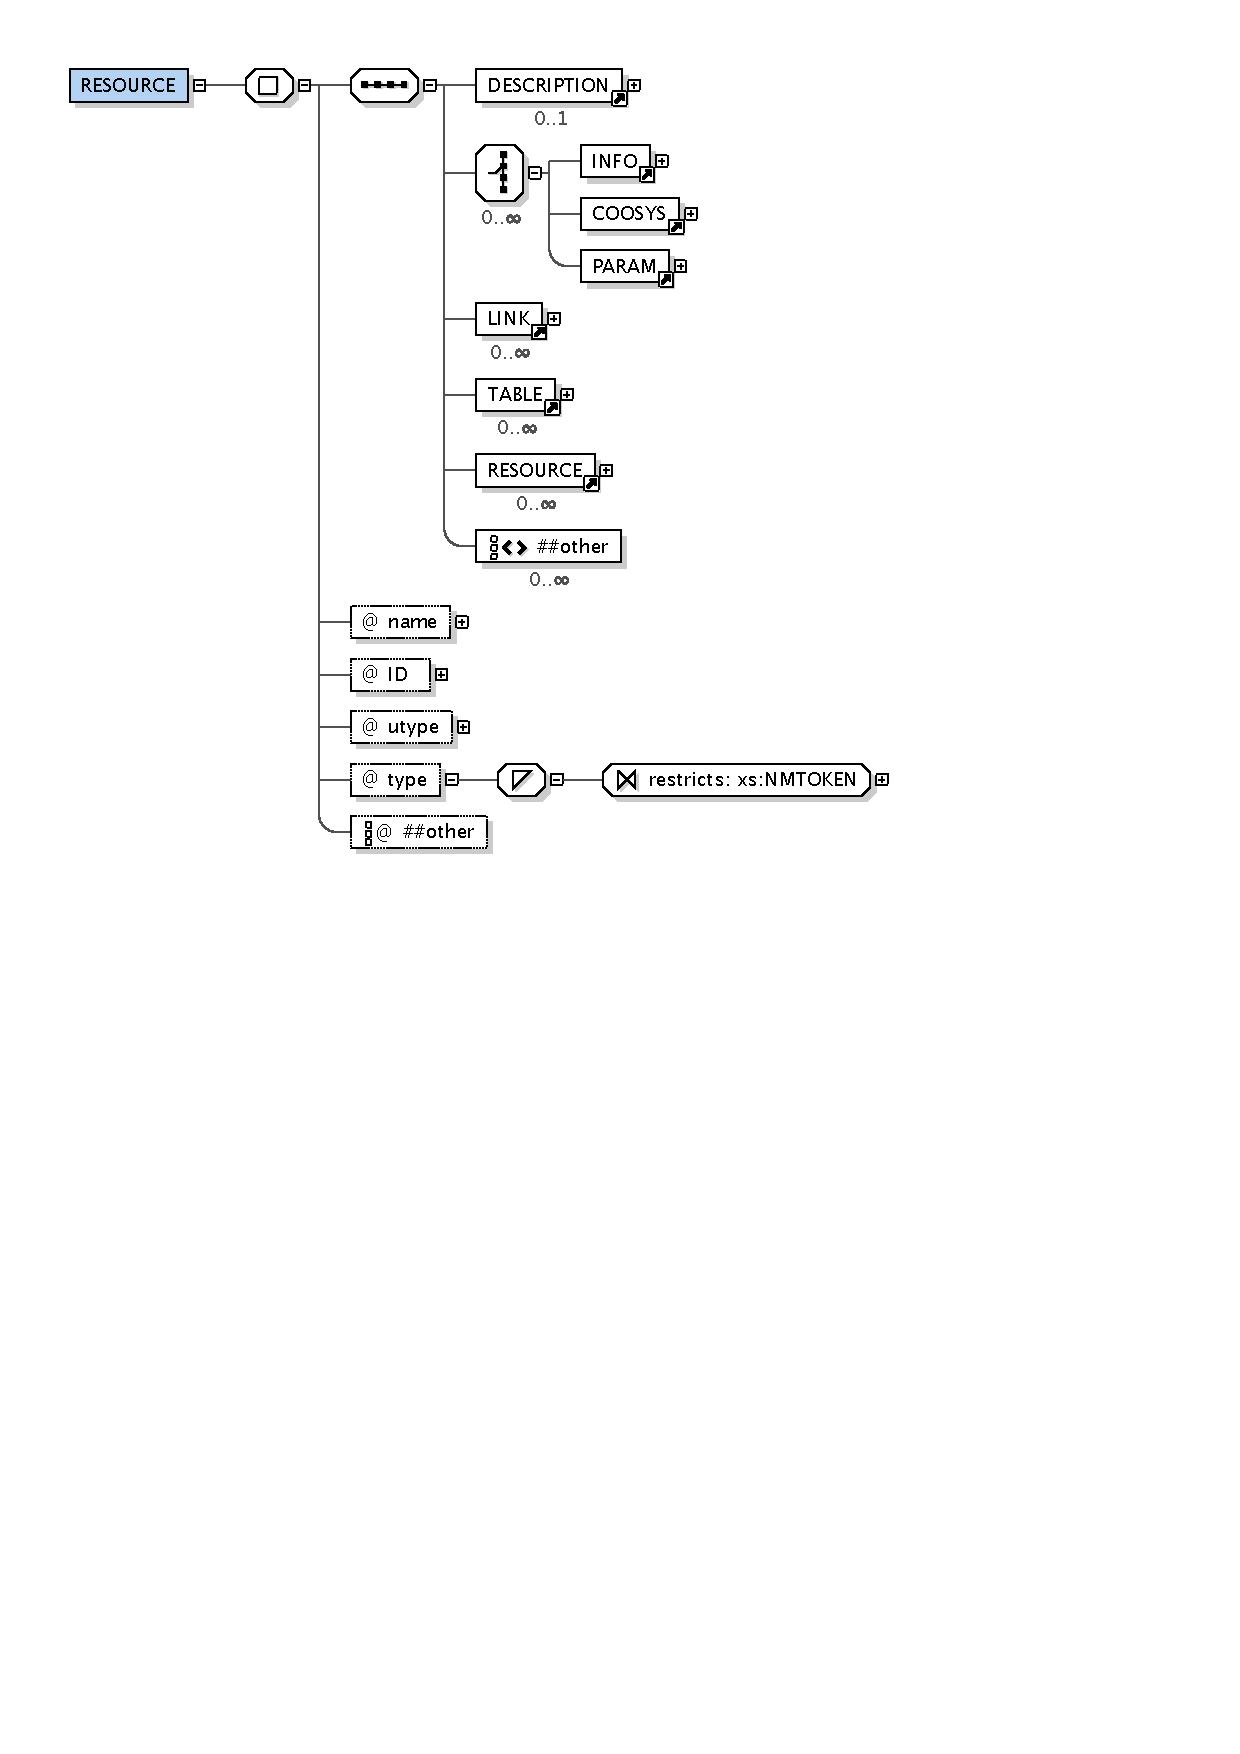
\includegraphics[width=\columnwidth]
		{fig/VOTableResourceTag.pdf}
	\caption[Elements of the \xmltag{RESOURCE}]{
		Elements of the \xmltag{RESOURCE}. \xmltags{RESOURCE} can
		contain many of the tags the \xmltag{VOTABLE} can hold, but
		additionally it can contain \xmlopen{LINK},\xmlopen{TABLE} and 
		\xmltags{RESOURCE}. \xmltags{TABLE} are used to include
		tabular data, while \xmltags{LINK} are used to point to
		non-tabular data resources being described by
		\xmlopen{DESCRIPTION}.
		\oxygenxml
	}
	\label{fig:fig_VOTableResourceTag}
\end{figure}



% subsection the_resource_tag (end)


\begin{figure}[tbp]
	\centering
		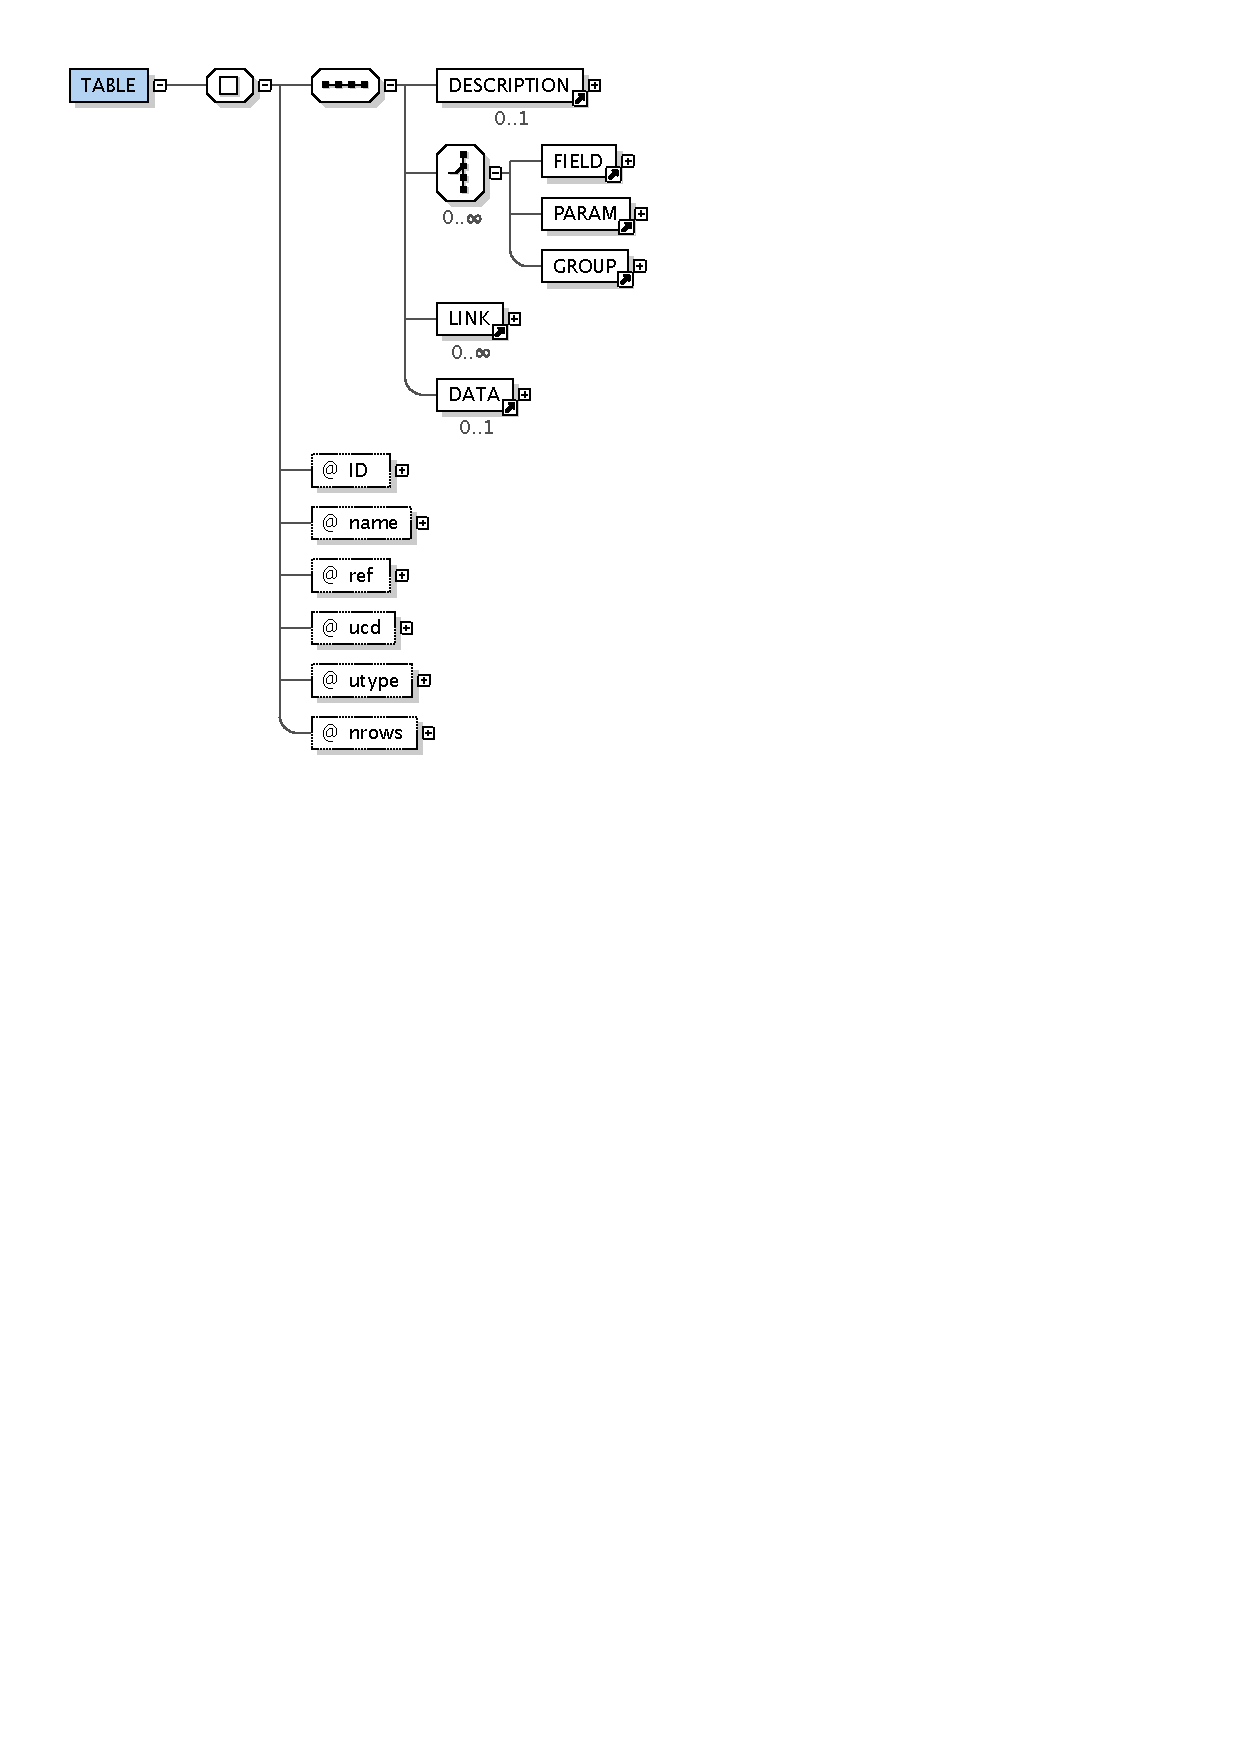
\includegraphics[scale=1]{fig/VOTableTableTag.pdf}
	\caption[Elements of the \xmltag{TABLE}]{
		Elements of the \xmltag{TABLE}. \xmltags{TABLE} might contain
		a \xmltag{DESCRIPTION}, and then they can be followed by
		any number of \xmlopen{FIELD}, \xmlopen{PARAM} and
		\xmltags{GROUP}. \xmltags{FIELD} are used to specify the
		different fields of the \xmlopen{DATA}, in case the VOTable
		contains inline data. Otherwise, the \xmltag{LINK} is used
		to reference remote data in other formats.
		The \xmltag{PARAM}
		is used to specify data which is common to all rows of the
		table, as if it were a \xmlopen{FIELD} whose value is the
		same for all rows. Finally, the \xmltag{GROUP} is used to
		group related fields or parameters, such as Right Ascension
		and Declination grouped into a coordinates \xmlopen{GROUP}.
		\oxygenxml
	}
	\label{fig:fig_VOTableTableTag}
\end{figure}

\begin{figure}[tbp]
	\centering
		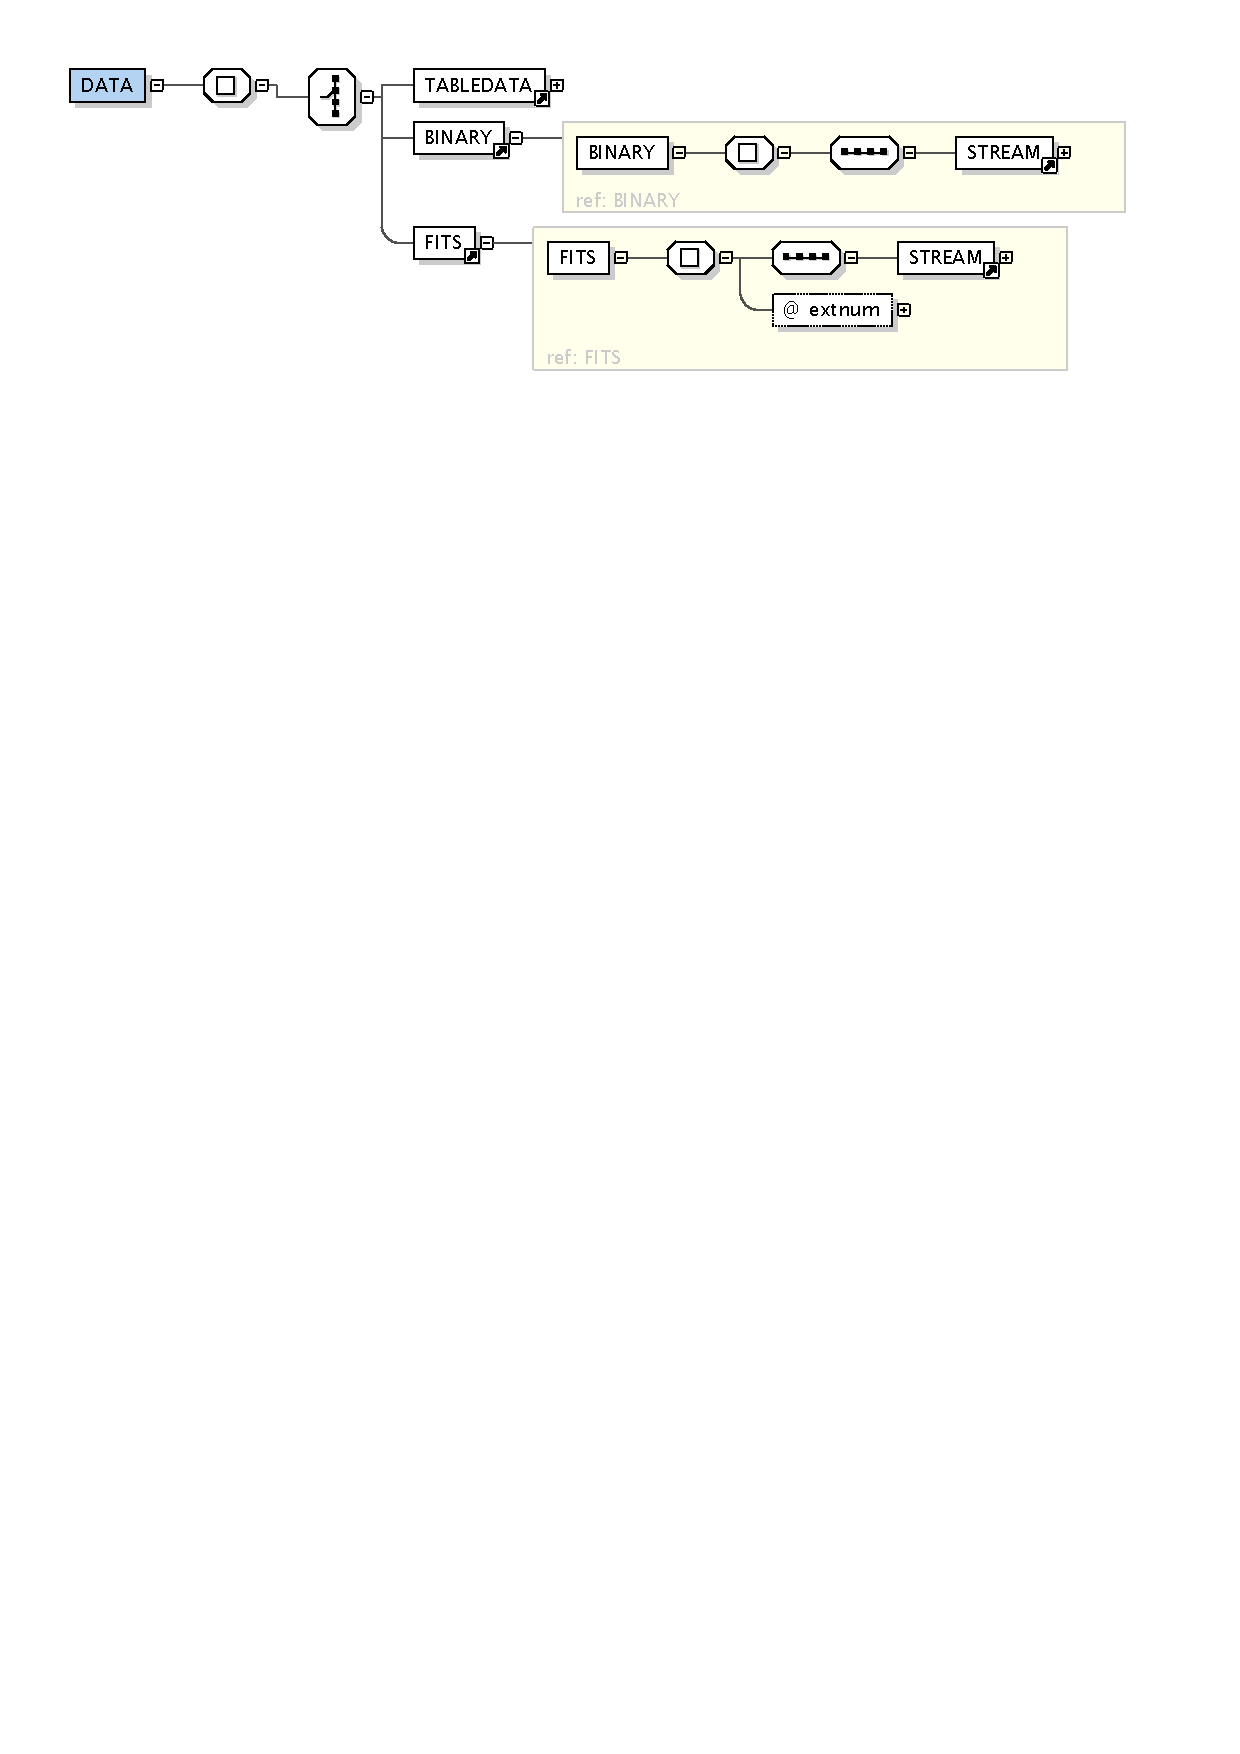
\includegraphics[width=\columnwidth]{fig/VOTableData.pdf}
	\caption[Elements of the \xmltag{DATA}]
	{
		Elements of the \xmltag{DATA}. In a \xmltag{RESOURCE},
		tabular information is included within a \xmltag{DATA}.
		That information can be pure XML tabular data within a
		\xmltag{TABLEDATA}, a linked FITS file within a \xmltag{FITS},
		or embedded binary data within \xmltag{BINARY}.
		The \xmltag{STREAM} contains either the data or references
		to the data. See figure~\ref{fig:fig_VOTableStream} for
		more information.
		\oxygenxml
	}
	\label{fig:fig_VOTableData}
\end{figure}

\begin{figure}[tbp]
	\centering
		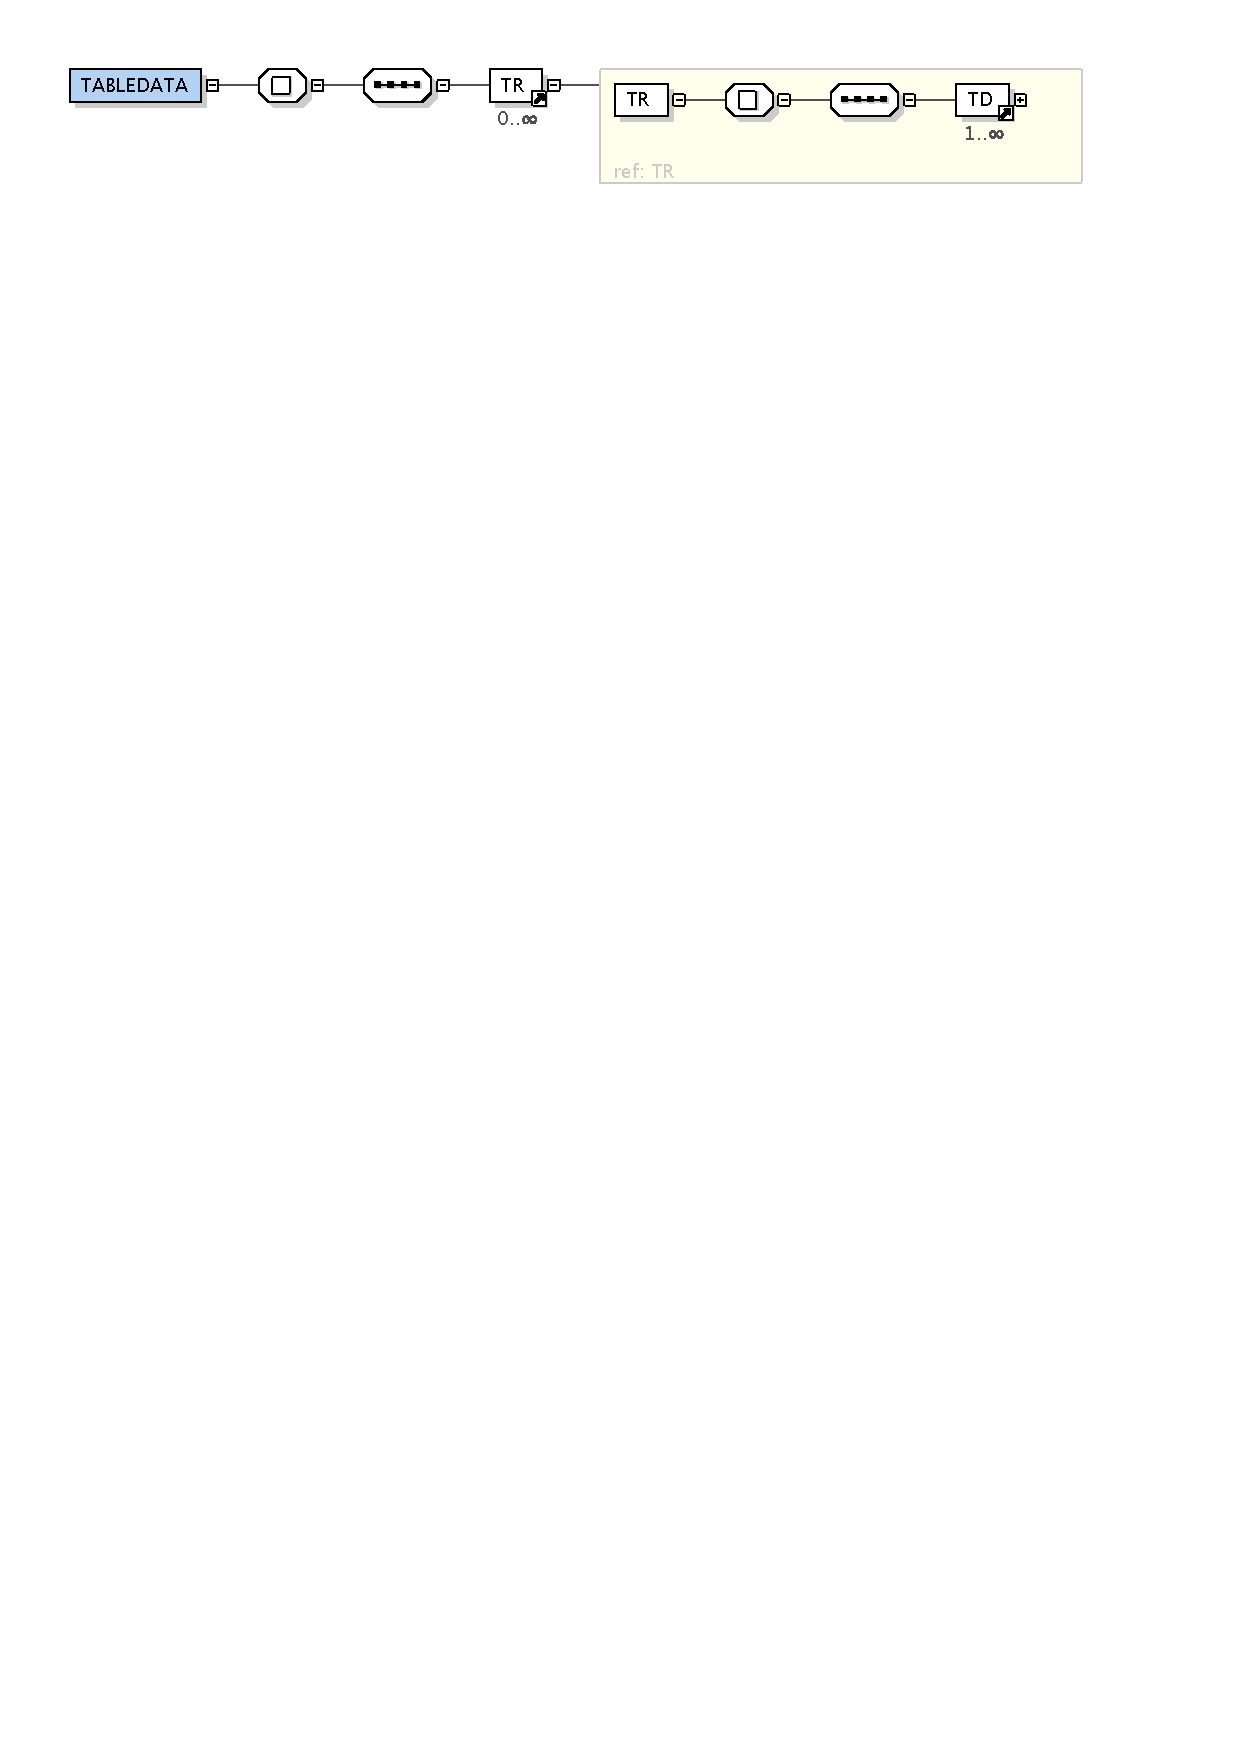
\includegraphics[width=\columnwidth]
		{fig/VOTableTabledataTag.pdf}
	\caption[Elements of the \xmltag{TABLEDATA}]{
		Elements of the \xmltag{TABLEDATA}. Inside the
		\xmltag{TABLEDATA} several \xmltags{TR} can exist,
		corresponding to different table rows. For each
		table row, there must be as many \xmltags{TD} as
		\xmltags{FIELD} in the \xmltag{TABLE} containing a
		particular \xmlopen{TABLEDATA}.
	}
	\label{fig:fig_VOTableTabledataTag}
\end{figure}


\begin{figure}[tbp]
	\centering
		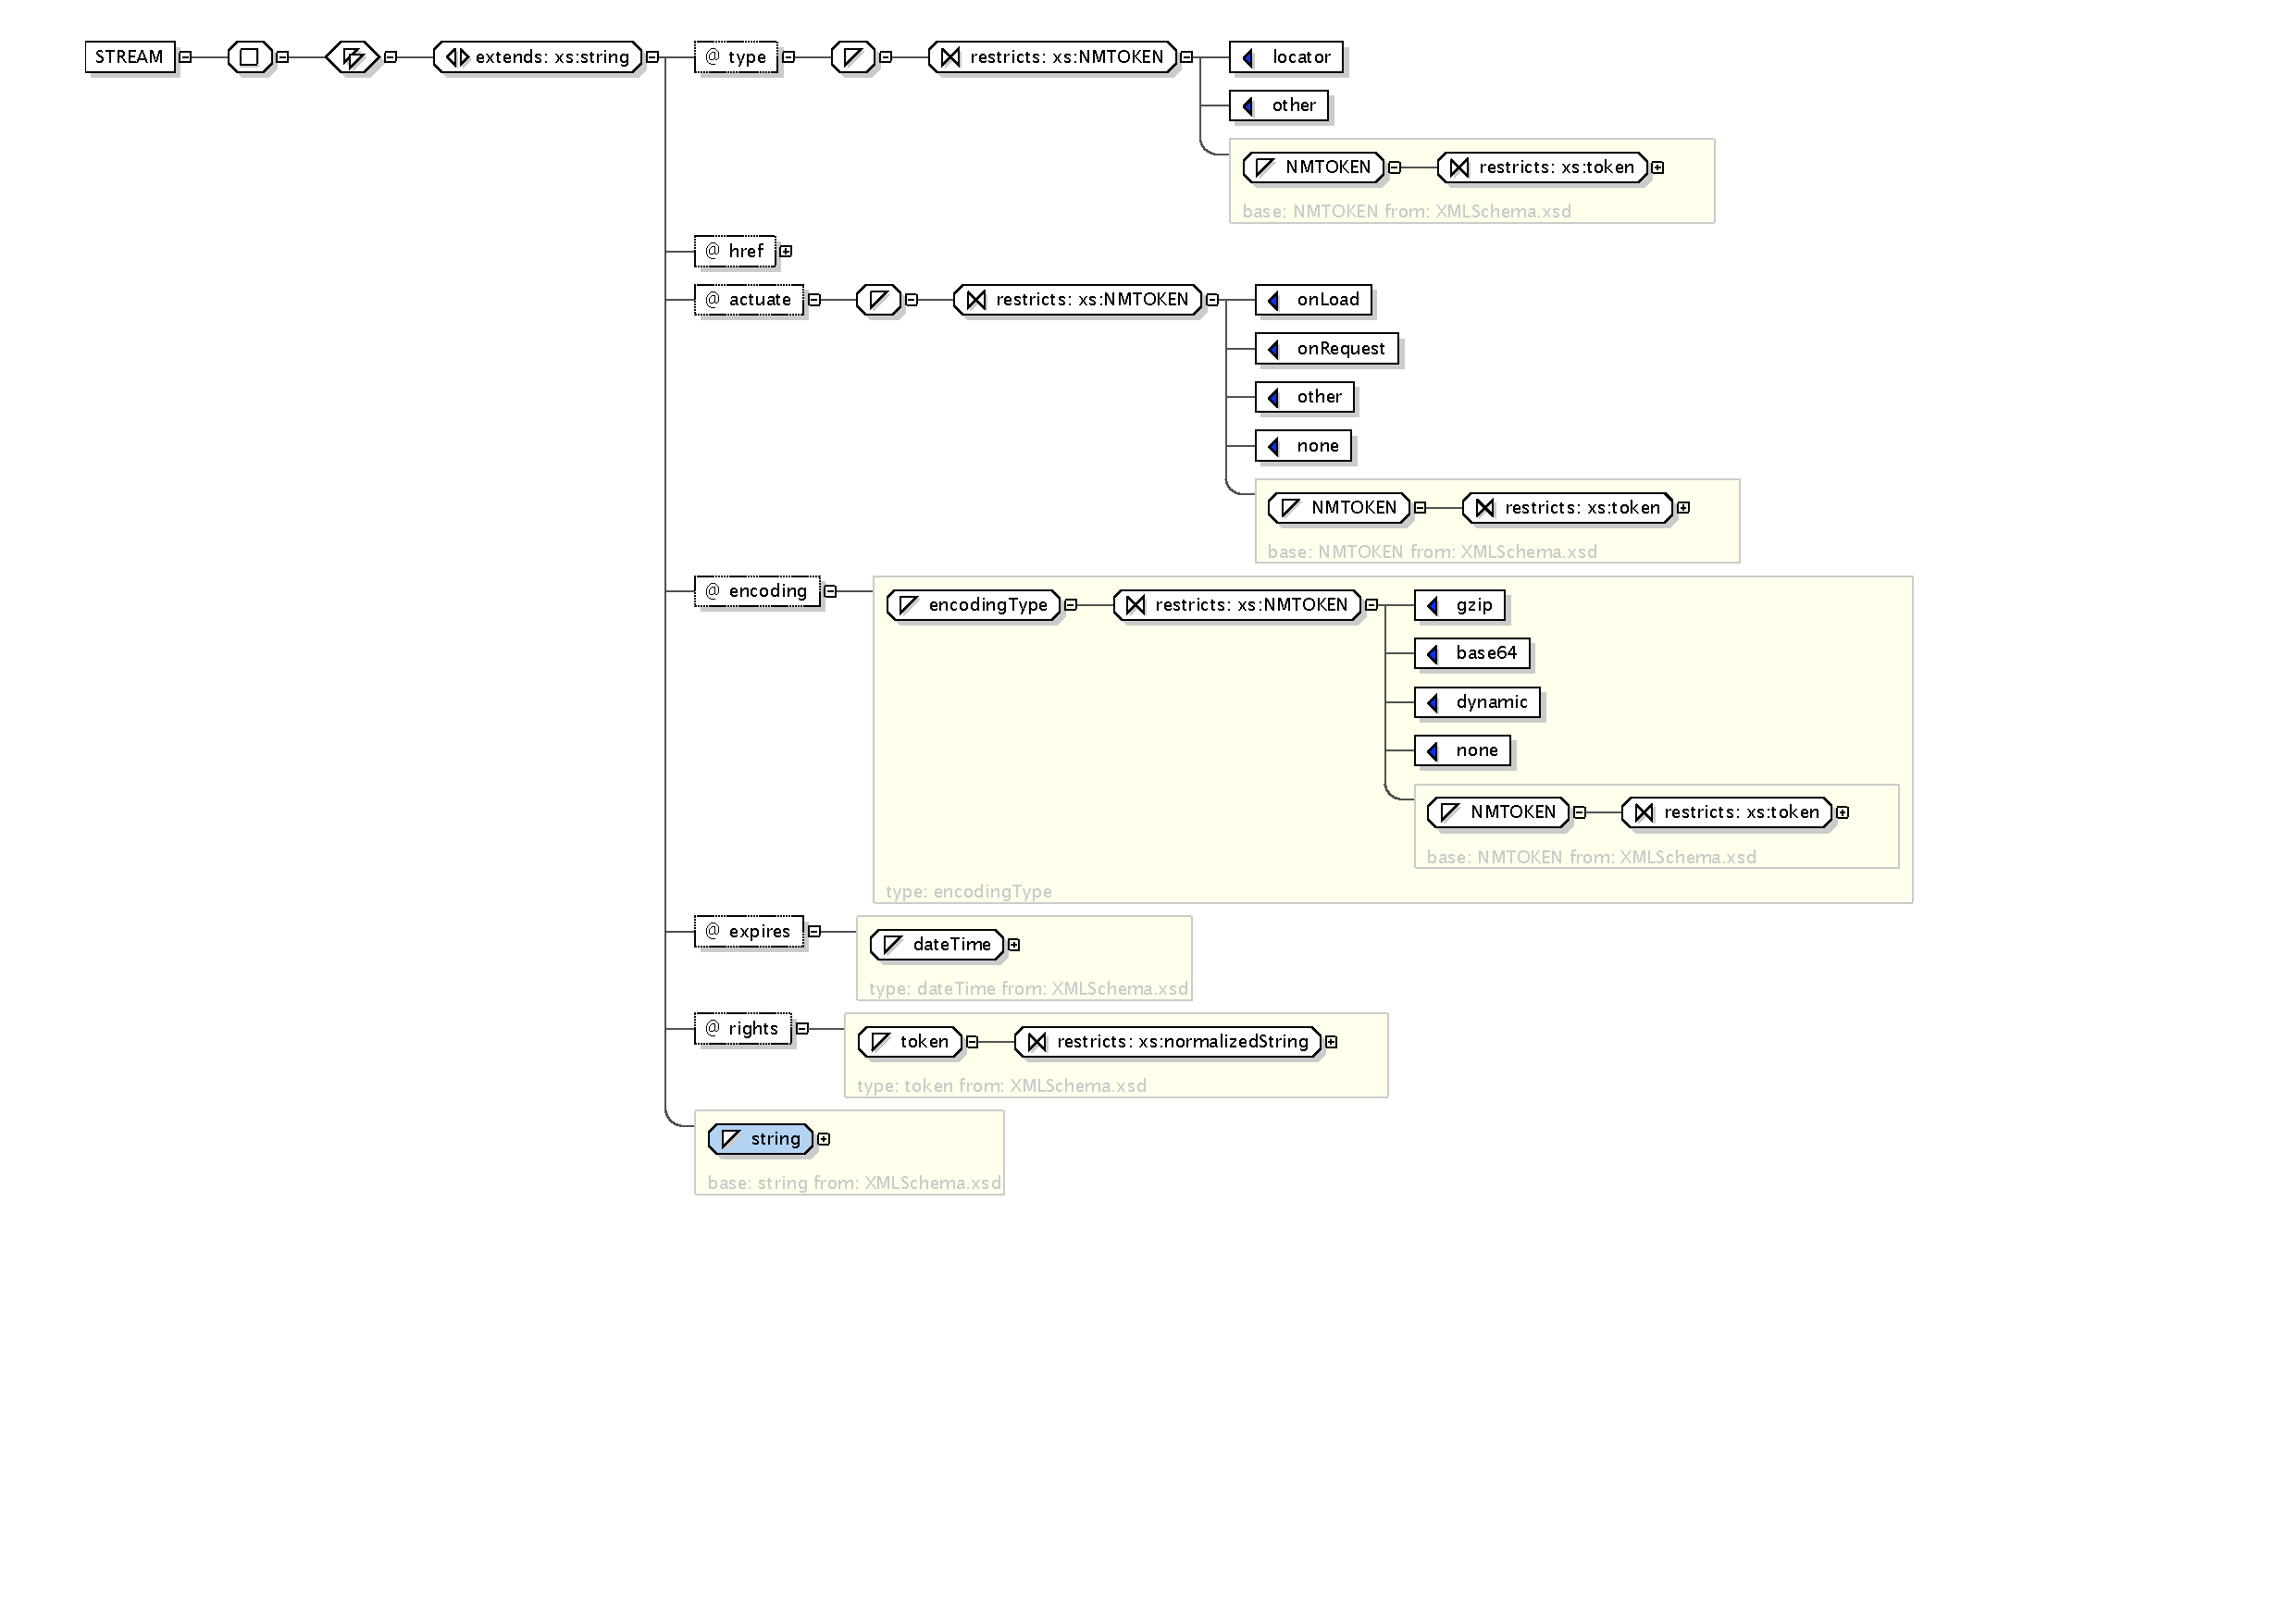
\includegraphics[width=\columnwidth]{fig/VOTableStream.pdf}
	\caption[Elements of the \xmltag{STREAM}]
	{
		Elements of the \xmltag{STREAM}. In this figure we have
		expanded the different attributes for the \xmltag{STREAM}
		in order to better understand what has to be provided. The
		\xmltag{STREAM} is a string which can contain data encoded
		in the formats specified by the \xmlattr{encoding}, only if
		the \xmlattr{type} is not \texttt{locator}. If the
		\xmlattr{type} were \texttt{locator}, the \xmlattr{href}
		would contain an URI pointing to the actual data source. In
		any case, an \xmlattr{expires} exists for transient
		datasets (for instance, on-demand synthetic datasets, image
		mosaics, or similar non-persistent datasets), the
		\xmlattr{actuate} exists for \todoinlinesuspended{Find out what is
		the \xmlattr{actuate} used for}, and the \xmlattr{rights}
		can be used to store a string (or an escaped XML fragment)
		which specifies in a human readable form the access rights
		for such data. \oxygenxml
	}
	\label{fig:fig_VOTableStream}
\end{figure}

% A complete diagram, comprising the whole schema tags and attributes,
% can be seen in figure~\ref{fig:fig_VOTable11-all}.

% \begin{figure}[tbp]
% 	\centering
% 		\includegraphics[width=\columnwidth,height=\textheight]
% 		{fig/VOTable11-all.png}
% 	\caption[VOTable 1.1 complete schema]
% 	{VOTable 1.1 diagram with all tags, attributes,
% 	and recursivity relationships.}
% 	\label{fig:fig_VOTable11-all}
% \end{figure}

\subsection{VOTable Data Types} % (fold)
\label{sub:votable_data_types}

In the following we will provide descriptions of the different
data types used within VOTables, together with their definition.

\subsubsection{\texttt{anyText}} % (fold)
\label{ssub:anytext}

\texttt{anyText} corresponds to a sequence of any characters of
indeterminate length, with the additional restriction that they must not
be processed in any way. This allows \texttt{anyText} elements to
be able to embed XHTML, or any other kind of textual content.

% subsubsection anytext (end)

\subsubsection{\texttt{astroYear}} % (fold)
\label{ssub:astroyear}

\texttt{astroYear} corresponds to a normalised string (a string
where white space is collapsed, and line-feeds are removed) which
conforms to the regular expression:

\begin{center}
	\texttt{[JB]?[0-9]+([.][0-9]*)?}
\end{center}

The regular expression considers as a valid \texttt{astroYear} any
string of one or more characters, optionally beginning either by
\texttt{J} or \texttt{B}, followed by any number (at least one) of
decimal digits, optionally followed by a decimal dot and any number of
decimal digits.

This pattern has been created with extensibility in mind, but the
most usual strings used for attributes with the \texttt{astroYear}
data type will be \texttt{B1950} and \texttt{J2000}.

% subsubsection astroyear (end)

\subsubsection{\texttt{ucdType}} % (fold)
\label{ssub:ucdtype}

\texttt{ucdType} corresponds to a normalised string which conforms
to the regular expression:

\begin{center}
	\verb![A-Za-z0-9_.;\-]*!
\end{center}

This regular expression considers as a valid \texttt{ucdType} any string
of any number of characters to choose any alphanumeric digit, string,
with the addition of the underscore (\texttt{\_}), the dot (\texttt{.}),
the semicolon (\texttt{;}), the backslash (\verb!\!) or the dash
(\texttt{-}). This pattern is valid for all UCDs in version 1.1, and for
most version 1 UCDs, even when these UCDs can make use of these symbols:
slash (\texttt{/}), plus (\texttt{+}) and percentage (\texttt{\%})
signs.

However, not all strings that match this pattern can be considered UCDs.
That is, matching the pattern is a necessary, but not sufficient,
precondition.

% subsubsection ucdtype (end)

\subsubsection{\texttt{arrayDEF}} % (fold)
\label{ssub:arraydef}

\texttt{arrayDEF} corresponds to a normalised string which conforms to
the regular expression:

\begin{center}
	\verb!([0-9]+x)*[0-9]*[*]?(s\W)?!
\end{center}

This regular expression considers a valid \texttt{arrayDEF} any string
formed by whole numbers separated by the eks character (\texttt{x}),
possibly followed by another whole number, possibly followed by an
asterisk (\texttt{*}), optionally followed by an s, and a non-word
character (neither letter nor digit).

This data type is used to specify textually multi-dimensional arrays
with defined dimensions, as in \texttt{12x512} for an array of 12 rows
and 512 columns, or \texttt{12x*} for an array of 12 rows and an
indeterminate number of columns.

When the \texttt{s} suffix is used, the non-word character is used to
specify the string separator. For instance, \texttt{1024s,} denotes an
array of strings, of up to 1024 characters in total, where the string
elements of the array are separated by a comma (\texttt{,}).

% subsubsection arraydef (end)

\subsubsection{\texttt{encodingType}} % (fold)
\label{ssub:encodingtype}

\texttt{encodingType} corresponds to one of the following strings:
\texttt{gzip}, \texttt{base64}, \texttt{dynamic}, or \texttt{none}.
Table~\ref{tab:encodingType_strings} shows the different meanings for
each string.

\begin{table}
	\caption[Valid \texttt{encodingType} attributes]{
		Meaning of the different valid values for attributes of the
		\texttt{encodingType} data type.
	}
	\begin{smallertabular}{rp{9.75cm}}
		\textbf{encodingType} & \textbf{Description} \\\midrule
		\texttt{gzip}    & Indicates that the link of the
		                   \xmltag{STREAM} has been compressed with
		                   \texttt{gzip}.\\\addlinespace
		\texttt{base64}  & Indicates a \texttt{base64} encoded link or
		                   embedded data.\\\addlinespace
		\texttt{dynamic} & Indicates that the stream encoding
		                   will be delivered dynamically when
		                   retrieving the link as part of the MIME
		                   type response.\\\addlinespace
		\texttt{none}    & No encoding other than that used for the
		                   VOTable is used.\\
	\end{smallertabular}
	\label{tab:encodingType_strings}
\end{table}

% subsubsection encodingtype (end)

\subsubsection{\texttt{dataType}} % (fold)
\label{ssub:datatype}

\texttt{dataType} corresponds to one of the following strings:
The string identifiers specify
data types for \xmlopen{FIELD} and \xmltags{PARAM}, as show in
table~\ref{tab:dataType_strings}


\begin{table}[btp]
	\begin{minipage}{\linewidth}
	\caption[Valid \texttt{dataType} attributes]{
		Meaning of the different valid values for 
		\texttt{dataType} identifiers, data range,
		and storage needs.
	}
	
	\begin{smallertabular}{rp{6.2cm}cc}
		    &   &
		\textbf{FITS} &  \\
		    &   &
		\textbf{equivalent} &  \\
		\textbf{Data type}    & \textbf{Description} &
		\textbf{type} & \textbf{Bytes} \\\midrule
		
		\texttt{boolean}	&	Boolean data,
							codified either as a \texttt{0} or
							\texttt{1} bit. & \texttt{L} & 1
							\\\addlinespace
							
		\texttt{bit}		&	Bitwise data
							(usually a bit array, corresponding to
							the FITS  type). Storage
							space is given in bytes for groups of
							8 bits. & \texttt{X} &
							$\ceil{b/8}$\footnote{Where $b$ is
							the number of bits in the bit array,
							and $\ceil{x}$ represents the nearest
							integer greater or equal to $x$.}
							\\\addlinespace
							
		\texttt{unsignedByte}
							& Unsigned integer number in the
							\texttt{0} to \texttt{255} range. & 
							\texttt{B} & 1
							\\\addlinespace
							
		\texttt{short}		& Signed integer number in
							the \texttt{-32768} to
							\texttt{32767} range. & \texttt{I} & 2
							\\\addlinespace
							
		\texttt{int}		&	Signed integer number in
							the \texttt{-2147483648} to
							\texttt{2147483647} range. & \texttt{J}
							& 4 \\\addlinespace
							
		\texttt{long}		& 	Signed integer number in the
							\texttt{-9223372036854775808} to 
							\texttt{9223372036854775807} range. &
							\texttt{K} & 8
							\\\addlinespace
							
		\texttt{char}		& Binary serialisation an ASCII (7-bit)
							character. & \texttt{A} & 1
							\\\addlinespace
							
		\texttt{unicodeChar}& Binary UTF-16 representation of a
							Unicode character. & n/a\footnote{There is
							no equivalence to the Unicode character
							in the FITS standard, which was developed
							much earlier than the Unicode standard.}
							& 2 \\\addlinespace
							
		\texttt{float}		& Binary ANSI/IEEE-754 32-bit floating
							point number in big-endian order. &
							\texttt{E} & 4
							\\\addlinespace
							
		\texttt{double}		& Binary ANSI/IEEE-754 64-bit double
							precision floating point number in
							big-endian order. & \texttt{D} & 8
							\\\addlinespace
							
		\texttt{floatComplex}
							& Pair of \texttt{float}, with the
							first element as the real part of the
							complex number, and the second as the
							imaginary part. & \texttt{C} & 8
							\\\addlinespace
							
		\texttt{doubleComplex}
							& Pair of \texttt{double}, with the
							first element as the real part of the
							complex number, and the second as the
							imaginary part. & \texttt{C} & 16
							\\\addlinespace
	\end{smallertabular}
	\label{tab:dataType_strings}
	\end{minipage}

\end{table}


% subsubsection datatype (end)

\subsubsection{\texttt{precType}} % (fold)
\label{ssub:prectype}

\texttt{precType} corresponds to a normalised string which conforms to
the regular expression:

\begin{center}
	\verb![EF]?[1-9][0-9]*!
\end{center}

This regular expression considers a valid \texttt{precType} any string
encoding an integer, without any leading zero, and optionally preceded
by an \texttt{E} or an \texttt{F} (which is the default). \texttt{F}
specifies a fixed digit precision, while \texttt{E} indicates a
relative precision.

For instance, \texttt{5} or \texttt{F5} indicates a fixed five decimal
digits precision, while \texttt{E5} specifies a relative precision of
$10^{-5}$, or 5 significant figures.


% subsubsection datatype (end)


% subsection votable_data_types (end)

% section votable_structure (end)




% chapter votable_format_definition (end)